\documentclass[11pt]{article}

\usepackage{fullpage}
\usepackage{graphicx}
\usepackage{amsmath}
\usepackage{amssymb}
\usepackage{amsthm}
\usepackage{fancyvrb}

\parindent0in
\pagestyle{plain}
\thispagestyle{plain}

\newcommand{\myname}{Mehshan Mustafa}
\newcommand{\dated}{\today}

\newenvironment{theorem}[2][Theorem]{\begin{trivlist}
\item[\hskip \labelsep {\bfseries #1}\hskip \labelsep {\bfseries #2.}]}{\end{trivlist}}
\newenvironment{lemma}[2][Lemma]{\begin{trivlist}
\item[\hskip \labelsep {\bfseries #1}\hskip \labelsep {\bfseries #2.}]}{\end{trivlist}}
\newenvironment{exercise}[2][Exercise]{\begin{trivlist}
\item[\hskip \labelsep {\bfseries #1}\hskip \labelsep {\bfseries #2.}]}{\end{trivlist}}
\newenvironment{problem}[2][Problem]{\begin{trivlist}
\item[\hskip \labelsep {\bfseries #1}\hskip \labelsep {\bfseries #2.}]}{\end{trivlist}}
\newenvironment{question}[2][Question]{\begin{trivlist}
\item[\hskip \labelsep {\bfseries #1}\hskip \labelsep {\bfseries #2.}]}{\end{trivlist}}
\newenvironment{corollary}[2][Corollary]{\begin{trivlist}
\item[\hskip \labelsep {\bfseries #1}\hskip \labelsep {\bfseries #2.}]}{\end{trivlist}}
\newenvironment{solution}{\begin{proof}[Solution]}{\end{proof}}
\newenvironment{idea}[2][Proof Idea.]{\textit{#1} #2}

\begin{document}

\textbf{Introduction to the Theory of
Computation}\hfill\textbf{\myname}\\[0.01in]
\textbf{Chapter 1: Reqular Languages}\hfill\textbf{\dated}\\
\smallskip\hrule\bigskip

\begin{problem}{1.66}
A homomorphism is a function $f : \Sigma \longrightarrow \Gamma^{*}$ from one alphabet to strings over another alphabet. We can extend $f$ to operate on strings by defining $f(w) = f(w_{1})f(w_{2}) \cdots f(w_{n})$, where $w = w_{1}w_{2} \cdots w_{n}$ and  each $w_{i} \in \Sigma$. We further
extend $f$ to operate on languages by defining $f(A) = \{f(w) \ | \ w \in A\}$, for any language A.
\end{problem}

\begin{problem}[Part]{a}
Show, by giving a formal construction, that the class of regular languages
is closed under homomorphism. In other words, given a DFA $M$ that recognizes $B$ and a homomorphism $f$, construct a finite automaton $M'$ that recognizes $f(B)$.
\end{problem}

\begin{idea}
Let $\Sigma = \{a, b\}$, $\Gamma = \{0, 1\}$, and $B = (ab)^{+}$. Define the homomorphism function $f$ on $\Sigma$ to be $f(a) = 11$, and $f(b) = 00$. Therefore, $f(ab) = 1100$ and $f(abab) = 11001100$.
\[ B = \{ab, abab, ababab, \cdots \}, and \ f(B) = \{1100, 11001100, 110011001100, \cdots \} \]
\begin{center}
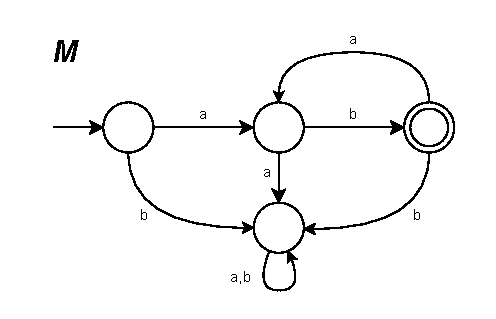
\includegraphics[scale=0.8]{Figures/Problem1.66a.pdf} \\
State diagram of the DFA $M$ that recognizes $B$.
\end{center}
\end{idea}

Next, construct a finite automaton $A_{f(a)}$ to recognize the string $f(a)$ for each $a \in \Sigma$. The DFA $M'$ to recognize $f(B)$ can be constructed by taking the DFA $M$ and by carrying out following steps for every transition between some initial state $q_{i}$ and subsequent state $q_{j}$ over some symbol $a$:
\begin{enumerate}
\item Remove the transition.
\item Add an $\epsilon$-transition that connects state $q_{i}$ to the start state of the DFA $A_{f(a)}$
\item Connect accept state of the DFA $A_{f(a)}$ with $q_{j}$ with an $\epsilon$-transition.
\item Make the accept state of $A_{f(a)}$ a non-accept state.
\end{enumerate}

\begin{center}
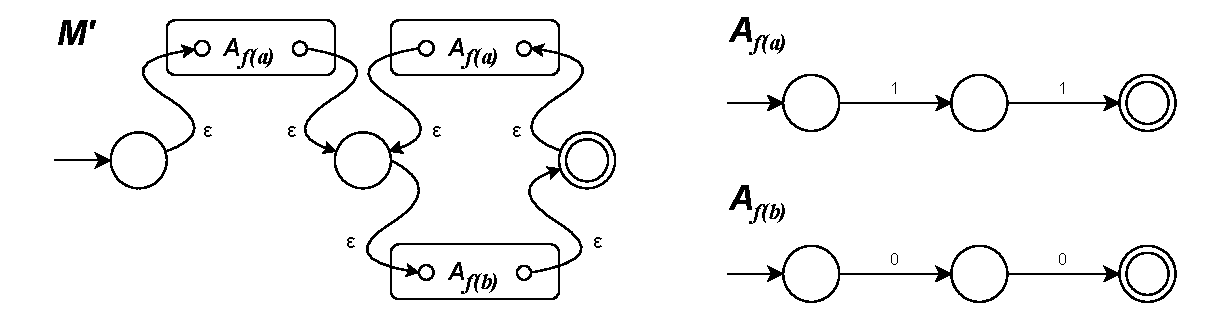
\includegraphics[scale=0.8]{Figures/Problem1.66b.pdf} \\
Construction of the NFA $M'$. Unnecessary transitions are omitted for simplicity.
\end{center}

\begin{proof}
Todo: provide formal construction using above idea.
\end{proof}

Consider the machine $M'$ that you constructed. Is it a DFA in every case?

If a given homomorphism function $f$ maps two different symbols in $\Sigma$ to a string over $\Gamma$ that starts with the same symbol then $M'$ can have non-deterministic tranisitions.

\begin{problem}[Part]{b}
Show, by giving an example, that the class of non-regular languages is not
closed under homomorphism.
\end{problem}

\begin{proof}
Solution Replace this text with the details of your proof or solution.
\end{proof}

\end{document}